\documentclass[lanscape, 10pt,twoside,a4paper]{article}
% http://www-h.eng.cam.ac.uk/help/tpl/textprocessing/latex_maths+pix/node6.html symboles de math
% http://fr.wikibooks.org/wiki/Programmation_LaTeX Programmation latex (wikibook)
%=========================== En-Tete =================================
%--- Insertion de paquetages (optionnel) ---
\usepackage[french]{babel}   % pour dire que le texte est en fran{\'e}ais
\usepackage{a4}	             % pour la taille   
\usepackage[T1]{fontenc}     % pour les font postscript
\usepackage{epsfig}          % pour gerer les images
%\usepackage{psfig}
\usepackage{amsmath, amsthm} % tres bon mode mathematique
\usepackage{amsfonts,amssymb}% permet la definition des ensembles
\usepackage{float}           % pour le placement des figure
\usepackage{verbatim}

\usepackage{multicol} % multicolonnes

\usepackage{longtable} % pour les tableaux de plusieurs pages

\usepackage[table]{xcolor} % couleur de fond des cellules de tableaux

\usepackage{lastpage}

\usepackage{multirow}

\usepackage{multicol} % pour {\'e}crire dans certaines zones en colonnes : \begin{multicols}{nb colonnes}...\end{multicols} 

% \usepackage[top=1.5cm, bottom=1.5cm, left=1.5cm, right=1.5cm]{geometry}
% gauche, haut, droite, bas, entete, ente2txt, pied, txt2pied
\usepackage{vmargin}
\setmarginsrb{0.20cm}{0.20cm}{0.20cm}{0.20cm}{15pt}{3pt}{42pt}{15pt}

	
\usepackage{pdflscape}
\usepackage{lscape} % changement orientation page
%\usepackage{frbib} % enlever pour obtenir references en anglais
% --- style de page (pour les en-tete) ---
\pagestyle{empty}

% mettre du texte en diagonale sur le fond : tikz
\usepackage{tikz} 
\def\confidentialTIKZ{%
	\begin{tikzpicture}[remember picture,overlay]
	\node[rotate=60,scale=15,text opacity=0.1] at (current page.center) {Confidentiel};
	\end{tikzpicture}
}%

\def\TIKZcyberpunkRED{%
	\begin{tikzpicture}[remember picture,overlay]
	\node[rotate=60,scale=10,text opacity=0.1] at (current page.center) {-- Cyberpunk RED};
	\end{tikzpicture}
}%

\usepackage{tikzpeople}

\def\txtTITLE{Feuille de personnage Cyberpunk RED} %%%%% !! TITRE !! %%%%%
\def\imgCORNER{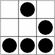
\includegraphics[width=0.25cm]{../../../../images/glider/logo-glider.png}}

\def\imgGLIDERLEFTT{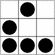
\includegraphics[width=1.95cm]{../../../../images/glider/logo-glider-left.png}}
\def\imgGLIDERRIGHT{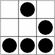
\includegraphics[width=1.95cm]{../../../../images/glider/logo-glider-right.png}}

\def\imgGLIDERLEFTTsmall{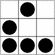
\includegraphics[width=0.25cm]{../../../../images/glider/logo-glider-left.png}}
\def\imgGLIDERRIGHTsmall{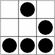
\includegraphics[width=0.25cm]{../../../../images/glider/logo-glider-right.png}}

% % % en-tete et pieds de page configurables : fancyhdr.sty

% http://www.trustonme.net/didactels/250.html

% http://ww3.ac-poitiers.fr/math/tex/pratique/entete/entete.htm
% http://www.ctan.org/tex-archive/macros/latex/contrib/fancyhdr/fancyhdr.pdf
\usepackage{fancyhdr}
\pagestyle{fancy}
	% \renewcommand{\chaptermark}[1]{\markboth{#1}{}}
	% \renewcommand{\sectionmark}[1]{\markright{\thesection\ #1}}
\fancyhf{}
\fancyhead[LE,RO]{\bfseries\thepage \TIKZcyberpunkRED }
\fancyhead[LO]{\bfseries\rightmark}
\fancyhead[RE]{\bfseries\leftmark}
\fancyfoot[LE]{\thepage /\pageref{LastPage} \hfill
	\scriptsize{\txtTITLE} % TITLE
\hfill \imgGLIDERLEFTTsmall }
\fancyfoot[RO]{\imgGLIDERRIGHTsmall \hfill
	\scriptsize{\txtTITLE} % TITLE
\hfill \thepage /\pageref{LastPage}}
\renewcommand{\headrulewidth}{0.5pt}
\renewcommand{\footrulewidth}{0.5pt}
\addtolength{\headheight}{0.5pt}
% \fancypagestyle{plain}{
	% \fancyhead{}
	% \renewcommand{\headrulewidth}{0pt}
% }

\def\smallbox{%
	\setlength{\unitlength}{0.5cm}
	\fbox{
		\begin{picture}(1, 1)(0,0)
		\end{picture}
	}
}%

%%%%%%%%%%% SOME VALUES IN ENGLISH %%%%%%%%%%%%%%%%%%%%%
%% \def\ENdefNom{\textbf{Name} \dotfill }

%%%%%%%%%%% 
\definecolor{verylightred}{rgb}{1.0,0.9,0.9}
\definecolor{lightred}{rgb}{1.0,0.75,0.75}
\definecolor{red}{rgb}{1.0,0.5,0.5}

\def\CELLredTXTWhite{\cellcolor{black} \color{white}}
\def\CELLredTXTWhite{\cellcolor{red} \color{black}}


%============================= Corps =================================
\begin{document}
\begin{landscape}

\setlength\parindent{0pt}

%% \small

\begin{tabular}{ p{0.20\textwidth} p{0.07\textwidth} p{0.32\textwidth} p{0.32\textwidth} p{0.32\textwidth} } 
	\begin{tabular}{ p{0.20\textwidth} }
		\footnotesize
		%% CyberPunk RED --- Fiche de personnage \\
		\fbox{ \begin{minipage}[ht]{0.20\textwidth} 
			-- 
			\newline \newline \newline \newline \newline 
			\newline \newline \newline \newline \newline
			\newline \newline \newline \newline \newline
		\end{minipage} } \\ 
		\fbox{ \begin{minipage}[ht]{0.20\textwidth} 
			Pseudo \newline
		\end{minipage} } \\ 
		\fbox{ \begin{minipage}[ht]{0.20\textwidth} 
			Rôle \newline
		\end{minipage} } \\ 
		\fbox{ \begin{minipage}[ht]{0.20\textwidth} 
			Capacité de Rôle	---	Rang \newline
		\end{minipage} } \\
		\fbox{ \begin{minipage}[ht]{0.20\textwidth}
			NOTES
			\newline \newline \newline \newline \newline
			\newline \newline \newline \newline \newline
		\end{minipage} } \\ 
		\fbox{ \begin{minipage}[ht]{0.20\textwidth} 
			Humanité	--- SUR --- \newline
		\end{minipage} } \\
	\end{tabular}
	& ~ 
	\begin{tabular}{ p{0.07\textwidth} }
		\footnotesize
		\fbox{ \begin{minipage}[ht]{0.07\textwidth} 
			INT \newline \newline 
		\end{minipage} } \\
		\fbox{ \begin{minipage}[ht]{0.07\textwidth} 
			RÉF \newline \newline 
		\end{minipage} } \\ 
		\fbox{ \begin{minipage}[ht]{0.07\textwidth} 
			DEX \newline \newline 
		\end{minipage} } \\ 
		\fbox{ \begin{minipage}[ht]{0.07\textwidth} 
			TECH \newline \newline 
		\end{minipage} } \\ 
		\fbox{ \begin{minipage}[ht]{0.07\textwidth} 
			PRES \newline \newline 
		\end{minipage} } \\ 
		\fbox{ \begin{minipage}[ht]{0.07\textwidth} 
			VOL \newline \newline 
		\end{minipage} } \\ 
		\fbox{ \begin{minipage}[ht]{0.07\textwidth} 
			CHA \newline \newline 
		\end{minipage} } \\ 
		\fbox{ \begin{minipage}[ht]{0.07\textwidth} 
			MOUV \newline \newline 
		\end{minipage} } \\ 
		\fbox{ \begin{minipage}[ht]{0.07\textwidth} 
			COR \newline \newline 
		\end{minipage} } \\ 
		\fbox{ \begin{minipage}[ht]{0.07\textwidth} 
			EMP \newline \newline 
		\end{minipage} } \\ 
	\end{tabular}
	& ~ 
	\begin{tabular}{ p{0.32\textwidth} }
		%% Table Compétence 1/3
		\fbox{ \begin{minipage}[ht]{0.32\textwidth}
			\footnotesize
			\begin{tabular}{|p{0.48\textwidth}|c|c|c|}
				\hline
				\CELLredTXTWhite 
				Compétences de Contrôle					&	NIV		&	CAR		&	BAS		\\
				\hline
				Conduite de véhicule Terrestre (RÉF)	&			&			&		 	\\
				\hline
				Équitation (RÉF)						&			&			&		 	\\
				\hline
				Pilotage de véhicule aérien (x2) (RÉF)	&			&			&		 	\\
				\hline
				Pilotage de véhicule maritime (RÉF)		&			&			&		 	\\
				\hline
			\end{tabular}

			\begin{tabular}{|p{0.48\textwidth}|c|c|c|}
				\hline
				\CELLredTXTWhite 
				Compétences \newline de Combat			&	NIV		&	CAR		&	BAS		\\
				\hline
				Arme de mêlée (DEX)						&			&			&		 	\\
				\hline
				Art martial (x2) (DEX)					&			&			&		 	\\
				\hline
				\textbf{Bagarre} (DEX)					&			&			&		 	\\
				\hline
				\textbf{Esquive} (DEX)					&			&			&		 	\\
				\hline
			\end{tabular}
			
			\begin{tabular}{|p{0.48\textwidth}|c|c|c|}
				\hline
				\CELLredTXTWhite 
				Compétences de Corps					&	NIV		&	CAR		&	BAS		\\
				\hline
				Athlétisme (DEX)						&			&			&		 	\\
				\hline
				Contorsion (DEX)						&			&			&		 	\\
				\hline
				Danse (DEX)								&			&			&		 	\\
				\hline
				\textbf{Discrétion} (DEX)				&			&			&		 	\\
				\hline
				Endurance (VOL)							&			&			&		 	\\
				\hline
				Résistance torture / drogues (VOL)		&			&			&		 	\\
				\hline
			\end{tabular}
			
			\begin{tabular}{|p{0.48\textwidth}|c|c|c|}
				\hline
				\CELLredTXTWhite 
				Compétences \newline d'Éducation		&	NIV		&	CAR		&	BAS		\\
				\hline
				Bibliothèque (INT)						&			&			&		 	\\
				\hline
				Bureaucratie (INT)						&			&			&		 	\\
				\hline
				Composition (INT)						&			&			&		 	\\
				\hline
				Comptabilité (INT)						&			&			&		 	\\
				\hline
				\textbf{Connaissance} (INT)				&			&			&		 	\\
				\hline
				Criminoologie (INT)						&			&			&		 	\\
				\hline
				Cryptographie (INT)						&			&			&		 	\\
				\hline
				Déduction (INT)							&			&			&		 	\\
				\hline
				Dressage (INT)							&			&			&		 	\\
				\hline
				Gestion d'affaires (INT)				&			&			&		 	\\
				\hline
				Jeux de hasard (INT)					&			&			&		 	\\
				\hline
			\end{tabular}
			%% --- 
		\end{minipage} } \\ 
	\end{tabular}
	& ~ 
	\begin{tabular}{ p{0.32\textwidth} }
		%% Table Compétence 2/3
		\fbox{ \begin{minipage}[ht]{0.32\textwidth}
			\footnotesize
			\begin{tabular}{|p{0.48\textwidth}|c|c|c|}
				\hline
				\CELLredTXTWhite 
				Compétences \newline d'Éducation		&	NIV		&	CAR		&	BAS		\\
				\hline
				Guide Local (INT)						&			&			&		 	\\
				\hline
				$\Rightarrow$ Quartier d'origine		&			&			&		 	\\
				\hline
				$\Rightarrow$ 							&			&			&		 	\\
				\hline
				$\Rightarrow$ 							&			&			&		 	\\				
				\hline
				Langue (INT)							&			&			&		 	\\
				\hline
				$\Rightarrow$ Argot						&			&			&		 	\\
				\hline
				$\Rightarrow$ 							&			&			&		 	\\
				\hline
				$\Rightarrow$ 							&			&			&		 	\\	
				\hline
				Science (INT)							&			&			&		 	\\
				\hline
				$\Rightarrow$ 							&			&			&		 	\\
				\hline
				$\Rightarrow$ 							&			&			&		 	\\	
				\hline
				Survie en milieu hostile (INT)			&			&			&		 	\\
				\hline
				Tactique (INT)							&			&			&		 	\\
				\hline				
			\end{tabular}
			
			\begin{tabular}{|p{0.48\textwidth}|c|c|c|}
				\hline
				\CELLredTXTWhite 
				Compétences \newline de représentration	&	NIV		&	CAR		&	BAS		\\
				\hline
				Instrument (TECH)						&			&			&		 	\\
				\hline
				$\Rightarrow$ 							&			&			&		 	\\
				\hline
				$\Rightarrow$ 							&			&			&		 	\\				
				\hline
				$\Rightarrow$ 							&			&			&		 	\\				
				\hline
				$\Rightarrow$ 							&			&			&		 	\\				
				\hline
				Jeu d'acteur (PRES)						&			&			&		 	\\
				\hline				
			\end{tabular}
			
			\begin{tabular}{|p{0.48\textwidth}|c|c|c|}
				\hline
				\CELLredTXTWhite 
				Compétences \newline de Sociabilité		&	NIV		&	CAR		&	BAS		\\
				\hline
				Connaissance de la rue (PRES)			&			&			&		 	\\
				\hline
				\textbf{Conversation} (EMP)				&			&			&		 	\\
				\hline
				Corruption (PRES)						&			&			&		 	\\
				\hline
				Habillement et Style (PRES)				&			&			&		 	\\
				\hline
				Interrogatoire (PRES)					&			&			&		 	\\
				\hline
				Look (PRES)								&			&			&		 	\\
				\hline
				Négoce (PRES)							&			&			&		 	\\
				\hline
				\textbf{Persuasion} (PRES)				&			&			&		 	\\
				\hline
				\textbf{Psychologie} (EMP)				&			&			&		 	\\
				\hline
			\end{tabular}
			%% --- 
		\end{minipage} } \\ 
	\end{tabular}
	& ~ 
	\begin{tabular}{ p{0.32\textwidth} }
		%% Table Compétence 3/3
		\fbox{ \begin{minipage}[ht]{0.32\textwidth}
			\footnotesize
			\begin{tabular}{|p{0.48\textwidth}|c|c|c|}
				\hline
				\CELLredTXTWhite 
				Compétences \newline de Technique		&	NIV		&	CAR		&	BAS		\\
				\hline
				Aérotech (TECH)							&			&			&		 	\\
				\hline
				Armurerie (TECH)						&			&			&		 	\\
				\hline
				Arts plastiques (TECH)					&			&			&		 	\\
				\hline
				Assistance médicale (x2) (TECH)			&			&			&		 	\\
				\hline
				Contrefaçon (TECH)						&			&			&		 	\\
				\hline
				Crochetage (TECH)						&			&			&		 	\\
				\hline
				Cybertech (TECH)						&			&			&		 	\\
				\hline
				Électronique (TECH)						&			&			&		 	\\
				\hline
				Explosifs (x2) (TECH)					&			&			&		 	\\
				\hline
				Maritech (TECH)							&			&			&		 	\\
				\hline
				Photos et films (TECH)					&			&			&		 	\\
				\hline
				Pickpocket (TECH)						&			&			&		 	\\
				\hline
				\textbf{Premier secours} (TECH)			&			&			&		 	\\
				\hline
				Sécurité électronique (x2) (TECH)		&			&			&		 	\\
				\hline
				Terratech (TECH)						&			&			&		 	\\
				\hline
			\end{tabular}
			
			\begin{tabular}{|p{0.48\textwidth}|c|c|c|}
				\hline
				\CELLredTXTWhite 
				Compétences de Tir						&	NIV		&	CAR		&	BAS		\\
				\hline
				Armes d'épaule (RÉF)					&			&			&		 	\\
				\hline
				Armes lourdes (x2) (RÉF)				&			&			&		 	\\
				\hline
				Pistolet (RÉF)							&			&			&		 	\\
				\hline
				Tir à l'arc (RÉF)						&			&			&		 	\\
				\hline
				Tir automatique (x2) (RÉF)				&			&			&		 	\\
				\hline
			\end{tabular}
			
			\begin{tabular}{|p{0.48\textwidth}|c|c|c|}
				\hline
				\CELLredTXTWhite 
				Compétences de~\newline Vigilance		&	NIV		&	CAR		&	BAS		\\
				\hline
				\textbf{Concentration} (VOL)			&			&			&		 	\\
				\hline
				Dissimulation / Révélation d'objet (INT)&			&			&		 	\\
				\hline
				Lecture sur les lèvres (INT)			&			&			&		 	\\
				\hline
				\textbf{Perception} (INT)				&			&			&		 	\\
				\hline
				Pistage (INT)							&			&			&		 	\\
				\hline
			\end{tabular}

			%% --- 
		\end{minipage} } \\ 
		
	\end{tabular}
	\\
	
	\hline \\ \hline
	
	\multicolumn{2}{ p{0.25\textwidth} }{
		%% Points de santé et blessures
		\begin{tabular}{|p{0.14\textwidth}|p{0.14\textwidth}|}
			\hline
			Points de santé	\newline									&	\multirow{2}{*}{Blessures Critiques}		\\
			\cline{1-1}
			Blessure Grave \newline										&												\\
			\hline
			\textbf{-2 à toutes les actions en \newline blessure grave}	&	\multirow{2}{*}{Addictions}					\\
			\cline{1-1}
			Sauvegarde contre la mort	\newline						&												\\		
			\hline
		\end{tabular}
	}
	& 
	\multicolumn{3}{ p{0.96\textwidth} }{
		--- 
		\begin{tabular}{|p{0.32\textwidth}|p{0.64\textwidth}|}
			\hline
			\textsc{\Large Armes et armures}			&		\multirow{2}{*}{
			\begin{tabular}{|p{0.10\textwidth}|p{0.10\textwidth}|p{0.10\textwidth}|p{0.10\textwidth}|p{0.10\textwidth}|} \hline
				\CELLredTXTWhite Arme		&	DG	&	Munitions	&	ATT/Round	&	Notes	\\ \hline
											&		&				&				&			\\ \hline
											&		&				&				&			\\ \hline
											&		&				&				&			\\ \hline
											&		&				&				&			\\ \hline
											&		&				&				&			\\ \hline
											&		&				&				&			\\ \hline
											&		&				&				&			\\ \hline
											&		&				&				&			\\ \hline
			\end{tabular} }											\\
			%% \hline
			\begin{tabular}{|p{0.08\textwidth}|p{0.08\textwidth}|p{0.08\textwidth}|} \hline
				\CELLredTXTWhite Armure		&	PA	&	Pénalité	\\ \hline
				Tête						&		&				\\ \hline
				Corps						&		&				\\ \hline
				Bouclier					&		&				\\ \hline
			\end{tabular} \newline \newline
			La pénalité s'applique à \newline RÉF, DEX et MOUV	
			 \newline \newline 									&	\\ \hline
		\end{tabular}
	}
	\\
	
\end{tabular}

\clearpage

%% DONE page 2 (parcours) (équipement)
~\\

\begin{tabular}{|p{0.46\textwidth}|p{0.85\textwidth}|} %% TOTAL : 131% in horizontal / landscape mode !! 
	%% PARCOURS 										&				ÉQUIPEMENT 								\\
	\hline
	\begin{tabular}{|p{0.20\textwidth}|p{0.20\textwidth}|}
		\hline
		\multicolumn{2}{|p{0.40\textwidth}|}{ Alias \newline \newline \newline }									\\
		\hline
		Points d'amélioration	 \newline 				&	\multirow{2}{*}{Évènements de réputation}				\\
		\cline{1-1}
		Réputation				 \newline 				&															\\
		\hline
		\multicolumn{2}{|p{0.40\textwidth}|}{ \textsc{\LARGE Parcours } }											\\
		\hline
		Origines culturelles \newline					&	Personnalité \newline									\\ \hline
		Tenue et coiffure \newline						&	Accessoire favori \newline								\\ \hline
		Valeur Fondamentale \newline					&	Que pensez vous des gens en général ? \newline			\\ \hline
		Àqui tenez vous le plus ? \newline				&	À quoi tenez vous le plus ? \newline					\\ \hline
		Originnes familliales \newline					&	Environnement \newline									\\ \hline
		Crise familiale \newline						&	But dans la vie \newline								\\ \hline
		Amis \newline									&	Tragédies amoureuses \newline							\\ \hline
		$\Rightarrow$ 	\newline 						&	$\Rightarrow$ 											\\ \hline
		$\Rightarrow$ 	\newline						&	$\Rightarrow$ 											\\ \hline
		$\Rightarrow$ 	\newline						&	$\Rightarrow$ 											\\ \hline
		\multicolumn{2}{ p{0.40\textwidth} }{ \footnotesize
			\begin{tabular}{|p{0.08\textwidth}|p{0.06\textwidth}|p{0.06\textwidth}|p{0.06\textwidth}|p{0.06\textwidth}|}
				Ennemis							&	Qui ?	&	Pourquoi ?	&	Actions~\footnote{Que peuvent-ils faire ?}		&	Futur~\footnote{Que va-t-il se passer ?}	\\ \hline
				$\Rightarrow$	\newline		&			&				&													&												\\ \hline
				$\Rightarrow$	\newline		&			&				&													&												\\ \hline
				$\Rightarrow$	\newline		&			&				&													&												\\ \hline
			\end{tabular}
		}
	\end{tabular}
	&
	\begin{tabular}{|p{0.20\textwidth}|p{0.55\textwidth}|} \hline
		\CELLredTXTWhite ÉQUIPEMENT	&	\CELLredTXTWhite NOTES		\\ \hline 
										&									\\ \hline
										&									\\ \hline
										&									\\ \hline
										&									\\ \hline
										&									\\ \hline
										&									\\ \hline
										&									\\ \hline
										&									\\ \hline
										&									\\ \hline
										&									\\ \hline
										&									\\ \hline
										&									\\ \hline
										&									\\ \hline
										&									\\ \hline
										&									\\ \hline
		\CELLredTXTWhite Munitions		&									\\ \hline
		\CELLredTXTWhite Eurodollars	&									\\ \hline
		
		\multicolumn{2}{ p{0.80\textwidth} }{ }	\\
		\multicolumn{2}{ p{0.80\textwidth} }{ }	\\
		\multicolumn{2}{ p{0.80\textwidth} }{ }	\\ 
		
		\hline \multicolumn{2}{|p{0.80\textwidth}|}{ 
			Style vestimentaire \newline \newline \newline
		} \\ \hline
		
		\multicolumn{2}{ p{0.80\textwidth} }{ }	\\
		\multicolumn{2}{ p{0.80\textwidth} }{ }	\\
		\multicolumn{2}{ p{0.80\textwidth} }{ }	\\ 
										
		\hline \multicolumn{2}{ p{0.80\textwidth} }{ 
			\begin{tabular}{|p{0.40\textwidth}|p{0.20\textwidth}|p{0.15\textwidth}|} \hline
				Logement \newline	&	Loyer \newline	&	Niveau de vie \newline \\ \hline
			\end{tabular}
		} \\ \hline

		\multicolumn{2}{ p{0.80\textwidth} }{ }	\\
		\multicolumn{2}{ p{0.80\textwidth} }{ }	\\
		\multicolumn{2}{ p{0.80\textwidth} }{ }	\\ 

		\hline \multicolumn{2}{|p{0.80\textwidth}|}{ 
			Parcours spécifique au rôle \newline \newline \newline
		} \\ \hline
	\end{tabular} \\
	\hline
\end{tabular}

\clearpage
	
%% DONE page 3 CYBERMATÉRIEL

%% TODO use tikz or custom image here !! 
%% see also "Custom "human" shape for tikz" https://tex.stackexchange.com/questions/84275/custom-human-shape-for-tikz
%% see also tikzpeople package : https://ctan.math.utah.edu/ctan/tex-archive/graphics/pgf/contrib/tikzpeople/tikzpeople.pdf and https://www.overleaf.com/latex/examples/quick-tikzpeople-example/gzbrzsdwtvtv

\begin{tabular}{|p{1.00\textwidth}|p{0.30\textwidth}|}

	\begin{tabular}{ p{0.30\textwidth} p{0.32\textwidth} p{0.30\textwidth} }
		&	
		\begin{tabular}{|p{0.14\textwidth}|p{0.14\textwidth}|} \hline
			\CELLredTXTWhite Kit Cyberaudio		&	\CELLredTXTWhite Données		\\ \hline 
												&									\\ \hline
												&									\\ \hline
												&									\\ \hline
		\end{tabular}	&	\\
		&	&	\\
		\begin{tabular}{|p{0.14\textwidth}|p{0.14\textwidth}|} \hline
			\CELLredTXTWhite Cyber\oe il gauche		&	\CELLredTXTWhite Données		\\ \hline 
													&									\\ \hline
													&									\\ \hline
													&									\\ \hline
		\end{tabular}
		&	&	
		\begin{tabular}{|p{0.14\textwidth}|p{0.14\textwidth}|} \hline
			\CELLredTXTWhite Cyber\oe il droit		&	\CELLredTXTWhite Données		\\ \hline 
													&									\\ \hline
													&									\\ \hline
													&									\\ \hline
		\end{tabular} \\
		&	&	\\
		\begin{tabular}{|p{0.14\textwidth}|p{0.14\textwidth}|} \hline
			\CELLredTXTWhite Cyberbras gauche	&	\CELLredTXTWhite Données		\\ \hline 
												&									\\ \hline
												&									\\ \hline
												&									\\ \hline
		\end{tabular}
		&	&	
		\begin{tabular}{|p{0.14\textwidth}|p{0.14\textwidth}|} \hline
			\CELLredTXTWhite Cyberbras droit	&	\CELLredTXTWhite Données		\\ \hline 
												&									\\ \hline
												&									\\ \hline
												&									\\ \hline
		\end{tabular} \\
		&	&	\\
		Pour un cyberimplant qui nécessite un cyberimplant de base (par exemple un cyber\oe il), cochez la case pour indiquer que vous avez l'implant de base. Inscrivez les extensions dans les lignes en dessous.~\newline &	
		\begin{tabular}{|p{0.14\textwidth}|p{0.14\textwidth}|} \hline
			\CELLredTXTWhite Câblage neural		&	\CELLredTXTWhite Données		\\ \hline 
												&									\\ \hline
												&									\\ \hline
												&									\\ \hline
												&									\\ \hline
												&									\\ \hline
												&									\\ \hline
		\end{tabular}	&	Pour un cyberimplant qui ne nécessite pas de cyberimplant de base (par exemple un cyberimplant interne), contentez-vous d'inscrire chaque cyberimplant dans les lignes en dessous du nom de la catégorie.~\newline	\\
		&	&	\\
		\begin{tabular}{|p{0.14\textwidth}|p{0.14\textwidth}|} \hline
			\CELLredTXTWhite Cyberjambe gauche		&	\CELLredTXTWhite Données		\\ \hline 
													&									\\ \hline
													&									\\ \hline
													&									\\ \hline
		\end{tabular}
		&	&	
		\begin{tabular}{|p{0.14\textwidth}|p{0.14\textwidth}|} \hline
			\CELLredTXTWhite Cyberjambe droite		&	\CELLredTXTWhite Données		\\ \hline 
													&									\\ \hline
													&									\\ \hline
													&									\\ \hline
		\end{tabular} \\
	
	\end{tabular}
	
	&
	\begin{tabular}{|p{0.10\textwidth}|p{0.10\textwidth}|} \hline
		\CELLredTXTWhite Cyberimplant interne	&	\CELLredTXTWhite Données		\\ \hline 
												&									\\ \hline
												&									\\ \hline
												&									\\ \hline
												&									\\ \hline
												&									\\ \hline
	\end{tabular} \newline 
	
	\begin{tabular}{|p{0.10\textwidth}|p{0.10\textwidth}|} \hline
		\CELLredTXTWhite Cyberimplant externe	&	\CELLredTXTWhite Données		\\ \hline 
												&									\\ \hline
												&									\\ \hline
												&									\\ \hline
												&									\\ \hline
												&									\\ \hline
	\end{tabular} \newline 
	
	\begin{tabular}{|p{0.10\textwidth}|p{0.10\textwidth}|} \hline
		\CELLredTXTWhite Cyberfashion		&	\CELLredTXTWhite Données		\\ \hline 
											&									\\ \hline
											&									\\ \hline
											&									\\ \hline
											&									\\ \hline
											&									\\ \hline
	\end{tabular} \newline 
	
	\begin{tabular}{|p{0.10\textwidth}|p{0.10\textwidth}|} \hline
		\CELLredTXTWhite Cyborgimplant		&	\CELLredTXTWhite Données		\\ \hline 
											&									\\ \hline
											&									\\ \hline
											&									\\ \hline
											&									\\ \hline
											&									\\ \hline
	\end{tabular} \newline 
	
	\begin{tikzpicture}
		\node[maninblack,evil,good,mirrored,monitor,saturated,shield,sword,minimum size=1.0cm]{One Evil ?};
		\node[sailor,evil,good,monitor,saturated,shield,sword,minimum size=1.0cm] at (3cm,0) {One AnOther ?};
	\end{tikzpicture} %% \newline  \newline  \newline 
	
	\\ \hline 
	
\end{tabular}

\end{landscape}

\end{document}
